% ============================================================================
%  W4A4 MMA-pipeline space-time diagram (standalone, compile with pdflatex)
%     pdflatex pipeline_spacetime.tex
% ============================================================================
\documentclass[border=6pt]{standalone}
\usepackage{tikz}
\usepackage{amsmath}
\usetikzlibrary{positioning,shapes,shadows,fit,backgrounds,arrows.meta,calc}

% ---- palette (paper-friendly, print-safe) ----------------------------------
\definecolor{hbmC}{RGB}{70,130,180}     % steel blue   - HBM cp.async
\definecolor{smemC}{RGB}{245,170, 90}   % warm orange  - SMEM prefetch
\definecolor{tcC}{RGB}{220, 90, 90}     % coral red    - Tensor Core MMA
\definecolor{epC}{RGB}{ 95,170,110}     % sage green   - FP32 epilogue fold
\definecolor{spC}{RGB}{150,100,200}     % violet       - sparse BSR branch
\definecolor{qC}{RGB}{ 90, 90, 90}      % grey         - activation quant
\definecolor{hlC}{RGB}{255,245,200}     % light yellow - overlap highlight

\begin{document}
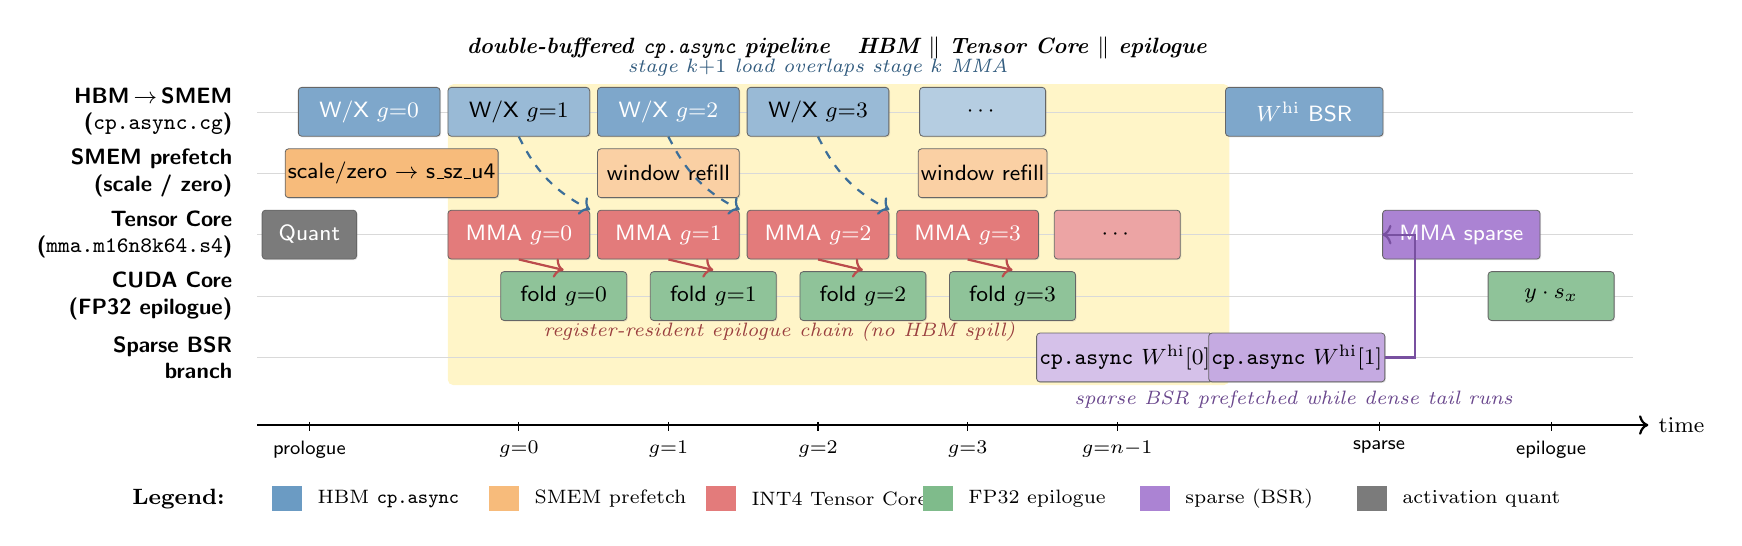
\begin{tikzpicture}[
  x=0.95cm, y=0.78cm,
  font=\footnotesize\sffamily,
  stage/.style={draw=black!60, line width=0.3pt, rounded corners=1.2pt,
                minimum height=0.62cm, align=center, inner sep=1pt,
                drop shadow={opacity=0.20, shadow xshift=0.4pt, shadow yshift=-0.4pt}},
  lane/.style ={font=\footnotesize\bfseries\sffamily, anchor=east, align=right},
  tick/.style ={font=\scriptsize\sffamily, anchor=north},
]

% ---------------- swim-lane labels -----------------------------------------
\node[lane] at (-0.2,  4) {HBM\,$\rightarrow$\,SMEM\\(\texttt{cp.async.cg})};
\node[lane] at (-0.2,  3) {SMEM prefetch\\(scale / zero)};
\node[lane] at (-0.2,  2) {Tensor Core\\(\texttt{mma.m16n8k64.s4})};
\node[lane] at (-0.2,  1) {CUDA Core\\(FP32 epilogue)};
\node[lane] at (-0.2,  0) {Sparse BSR\\branch};

% horizontal lane guides
\foreach \y in {0,1,2,3,4}
  \draw[black!15, line width=0.2pt] (0,\y) -- (18.4,\y);

% ---------------- time axis ------------------------------------------------
\draw[->, thick] (0,-1.1) -- (18.6,-1.1) node[right, font=\footnotesize] {time};
\foreach \t/\lbl in {0.7/prologue, 3.5/{$g{=}0$}, 5.5/{$g{=}1$}, 7.5/{$g{=}2$},
                      9.5/{$g{=}3$}, 11.5/{$g{=}n{-}1$}, 15.0/{sparse}, 17.3/{epilogue}}
  \draw (\t,-1.05) -- (\t,-1.20) node[tick] {\lbl};

% ---------------- overlap-highlight band (drawn first, behind) -------------
\begin{scope}[on background layer]
  \fill[hlC, rounded corners=2pt] (2.55, -0.45) rectangle (13.00, 4.45);
  \node[font=\footnotesize\itshape\bfseries, anchor=south]
    at (7.75, 4.70)
    {double-buffered \texttt{cp.async} pipeline \ \ HBM $\parallel$ Tensor Core $\parallel$ epilogue};
\end{scope}

% ---------------- lane 4 : HBM cp.async (double-buffered) ------------------
\node[stage, fill=hbmC!70, text=white] (h0) at (1.5,  4) [minimum width=1.8cm]{W/X $g{=}0$};
\node[stage, fill=hbmC!55]             (h1) at (3.5,  4) [minimum width=1.8cm]{W/X $g{=}1$};
\node[stage, fill=hbmC!70, text=white] (h2) at (5.5,  4) [minimum width=1.8cm]{W/X $g{=}2$};
\node[stage, fill=hbmC!55]             (h3) at (7.5,  4) [minimum width=1.8cm]{W/X $g{=}3$};
\node[stage, fill=hbmC!40]             (hd) at (9.7,  4) [minimum width=1.6cm]{$\cdots$};
\node[stage, fill=hbmC!70, text=white] (hs) at (14.0, 4) [minimum width=2.0cm]{$W^{\mathrm{hi}}$ BSR};

% ---------------- lane 3 : SMEM prefetch -----------------------------------
\node[stage, fill=smemC!80] at (1.8, 3) [minimum width=2.4cm]{scale/zero $\rightarrow$ s\_sz\_u4};
\node[stage, fill=smemC!55] at (5.5, 3) [minimum width=1.8cm]{window refill};
\node[stage, fill=smemC!55] at (9.7, 3) [minimum width=1.6cm]{window refill};

% ---------------- lane 2 : Tensor Core MMA ---------------------------------
\node[stage, fill=qC!80, text=white]   (q)  at (0.7, 2) [minimum width=1.2cm]{Quant};
\node[stage, fill=tcC!80, text=white]  (t0) at (3.5, 2) [minimum width=1.8cm]{MMA $g{=}0$};
\node[stage, fill=tcC!80, text=white]  (t1) at (5.5, 2) [minimum width=1.8cm]{MMA $g{=}1$};
\node[stage, fill=tcC!80, text=white]  (t2) at (7.5, 2) [minimum width=1.8cm]{MMA $g{=}2$};
\node[stage, fill=tcC!80, text=white]  (t3) at (9.5, 2) [minimum width=1.8cm]{MMA $g{=}3$};
\node[stage, fill=tcC!55]              (td) at (11.5,2) [minimum width=1.6cm]{$\cdots$};
\node[stage, fill=spC!80, text=white]  (ts) at (16.1,2) [minimum width=2.0cm]{MMA sparse};

% ---------------- lane 1 : FP32 epilogue fold  (d - z*sum)*s ---------------
\node[stage, fill=epC!70] (f0) at (4.1,  1) [minimum width=1.6cm]{fold $g{=}0$};
\node[stage, fill=epC!70] (f1) at (6.1,  1) [minimum width=1.6cm]{fold $g{=}1$};
\node[stage, fill=epC!70] (f2) at (8.1,  1) [minimum width=1.6cm]{fold $g{=}2$};
\node[stage, fill=epC!70] (f3) at (10.1, 1) [minimum width=1.6cm]{fold $g{=}3$};
\node[stage, fill=epC!70] (fe) at (17.3, 1) [minimum width=1.6cm]{$y \cdot s_x$};

% ---------------- lane 0 : sparse branch prefetch --------------------------
\node[stage, fill=spC!40] (sp0) at (11.6, 0) [minimum width=1.8cm]{\texttt{cp.async} $W^{\mathrm{hi}}[0]$};
\node[stage, fill=spC!55] (sp1) at (13.9, 0) [minimum width=1.8cm]{\texttt{cp.async} $W^{\mathrm{hi}}[1]$};

% ---------------- dependency arrows (key overlap edges) --------------------
\draw[->, thick, hbmC!85!black, dashed] (h1.south) to[bend right=18] (t0.north east);
\draw[->, thick, hbmC!85!black, dashed] (h2.south) to[bend right=18] (t1.north east);
\draw[->, thick, hbmC!85!black, dashed] (h3.south) to[bend right=18] (t2.north east);

\draw[->, thick, tcC!85!black] (t0.south) -- ($(f0.north)+(0,0.02)$);
\draw[->, thick, tcC!85!black] (t1.south) -- ($(f1.north)+(0,0.02)$);
\draw[->, thick, tcC!85!black] (t2.south) -- ($(f2.north)+(0,0.02)$);
\draw[->, thick, tcC!85!black] (t3.south) -- ($(f3.north)+(0,0.02)$);

% dense -> sparse transition arrow
\draw[->, thick, spC!80!black] (sp1.east) -- ++(0.4,0) |- (ts.west);

% ---------------- annotations (the "pipeline storytelling" labels) ---------
\node[font=\scriptsize\itshape, text=hbmC!70!black, anchor=south]
  at (7.50, 4.42) {stage $k{+}1$ load overlaps stage $k$ MMA};
\node[font=\scriptsize\itshape, text=tcC!70!black, anchor=west]
  at (3.70, 0.42) {register-resident epilogue chain  (no HBM spill)};
\node[font=\scriptsize\itshape, text=spC!70!black, anchor=west]
  at (10.8, -0.68) {sparse BSR prefetched while dense tail runs};

% ---------------- legend ---------------------------------------------------
\begin{scope}[shift={(0, -2.5)}]
  \node[anchor=east, font=\footnotesize\bfseries] at (-0.3, 0.2) {Legend:};
  \foreach \i/\c/\lbl in {0/hbmC/{HBM \texttt{cp.async}},
                          1/smemC/{SMEM prefetch},
                          2/tcC/{INT4 Tensor Core},
                          3/epC/{FP32 epilogue},
                          4/spC/{sparse (BSR)},
                          5/qC/{activation quant}} {
    \fill[\c!80] (\i*2.9+0.2, 0) rectangle ++(0.4, 0.4);
    \node[anchor=west, font=\scriptsize] at (\i*2.9+0.68, 0.2) {\lbl};
  }
\end{scope}

\end{tikzpicture}
\end{document}
